\documentclass[]{article}
\usepackage{algpseudocode}
\usepackage{tikz}
\usepackage{pgfplots}
\usetikzlibrary{positioning}

\pagenumbering{roman}

\title{Time Complexity, Data Structures, Sorts and Searches}
\author{D\'{a}rio Tavares Antunes}
\date{}

\newcommand{\numberLess}[1]{
\addcontentsline{toc}{section}{#1}
\section*{#1}
}

\newcommand{\subNumberLess}[1]{
\addcontentsline{toc}{section}{#1}
\subsection*{#1}
}

\begin{document}
	
\maketitle

\tableofcontents

\pagebreak
\pagenumbering{arabic}

\numberLess{Big-O Notation}

A quick, more formal definition than follows below can be stated as - some function $f(n)$ has a time complexity $g(n)$ (that is, it is of $O(g(n))$) if and only if:

\[\lim_{n \to +\infty}\frac{f(n)}{g(n)} < \infty\]

Big-O notation defines how the time taken to complete a task scales with the size of your input. It describes the asymptotic behaviour of functions. That is, as n increases to a large value (generally $+\infty$).

It takes only the largest contributing term of the polynomial describing the time complexity of a given function. These follow the inequality below:

\[n! > c^{n} > n^{k} > n^{k-1} > n\log{n} > n > \log{n} > 1\]

A graphical representation can be found in Figure \ref{fig:time} on page \pageref{fig:time}. Note that these functions are only sampled (or at least I tried to only sample them) at integer values, as n will always be a natural number.

These time complexities are called, respectively; factorial, exponential, polynomial (twice), linearithmic (not a very common name), linear, logarithmic and constant. The reason for these should, hopefully, be obvious.

Calculating the time complexity of a function cannot be done mechanically, due to the halting problem. Thus, analysis of the function must be done by hand. Take the example of the code below

\begin{algorithmic}[1]
	\State $values \gets randomArrayOfLength(n)$
	\State $total \gets 0$
	\For{\emph{each value in values}}
		\State $total \gets total + value$
	\EndFor
\end{algorithmic}

For the sake of the example, let's assume the \emph{randomArrayOfLength()} function has $O(n)$ time complexity, generating a number in constant time and doing this $n$ times. $n \times 1 = n$ and so the it is $O(n)$. We assign a value of n to this line.

We assume that assigning a variable occurs in constant time on the next line and give it a value of 1.

Finally, the for loop. We first calculate the time complexity of its inner operations, then multiply it by the number of times the loop runs. As assigning the variable is constant time and, presumably, so is adding the values, we assign a value of 1.

The loop completes once for each value, which is to say n times. It is therefore $O(n)$.

We then add these values to obtain a polynomial representing the time complexity of the function, $T(n) = 2n + 1$. The highest order is n, and so the function has $O(n)$ time complexity.

\begin{figure}
\centering
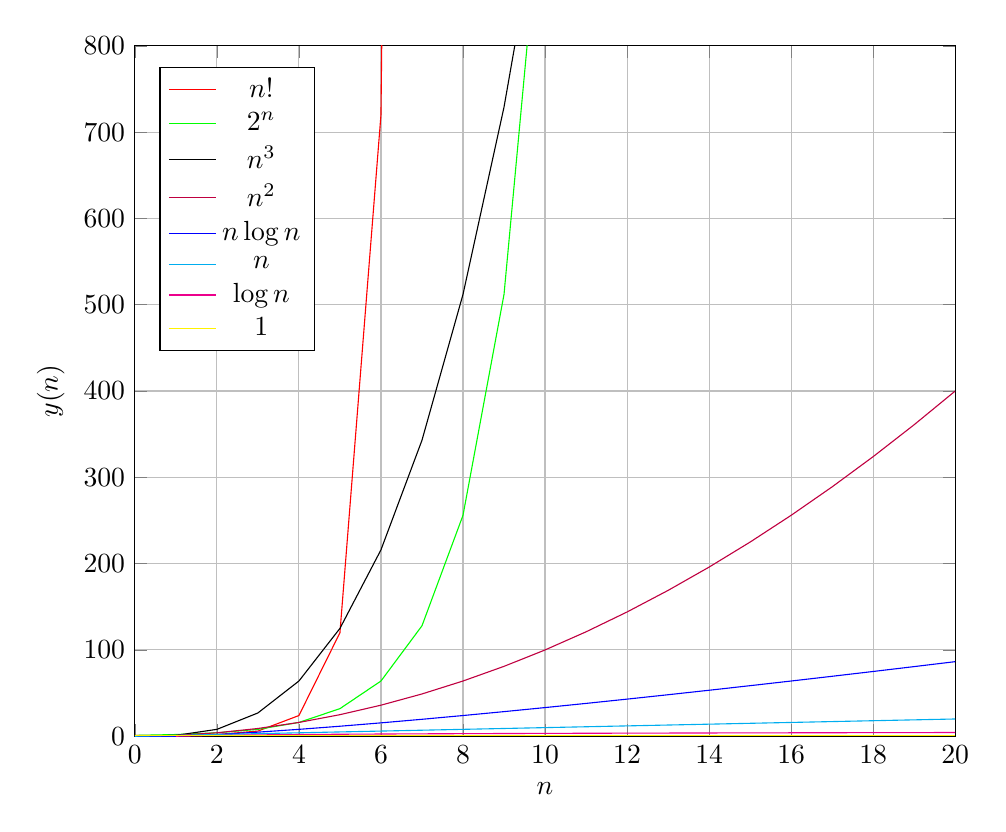
\begin{tikzpicture}
\begin{axis}[domain=0:20, samples=21,grid=major,ymin=0,ymax=800,xmin=0,xmax=20,
    restrict y to domain=0:10000,
    xlabel=$n$,ylabel=$y(n)$, legend pos=north west, width=12cm]
\addplot [color=red]    {factorial(x)};
\addplot [color=green]  {pow(2, x)};
\addplot [color=black] {pow(x, 3)}; 
\addplot [color=purple] {pow(x, 2)}; 
\addplot [color=blue]   {x * log2(x)};
\addplot [color=cyan] {x}; 
\addplot [color=magenta] {log2(x)}; 
\addplot [color=yellow] {1}; 

\legend{$n!$, $2^n$, $n^3$, $n^2$, $n\log{n}$, $n$, $\log{n}$, $1$}
\end{axis}
\end{tikzpicture}
\caption{Time Complexities}
\label{fig:time}
\end{figure}

\pagebreak

\section{Data Structures}

\subsection{Array Backed}

\subsubsection{Basic Array}

The default array structure, with its size fixed when it's initiated/allocated. While this makes it inflexible in some senses relative to other data structures, it has certain benefits.

Indexing is $O(1)$, as elements are stored congruously in memory and accessed by offset.

However, in the general case, the worst case for searching the array is $O(n)$ as every element must be checked. This can be reduced by sorting the array if the current ordering is not important, however.

Unlike other data structures, insertion and deletion are not supported, every index must contain something. If the array is not allocated well, it may waste space with unfilled indices. However, its space complexity should only be $O(n)$.

\subsubsection{Dynamic Array}

This is a list allowing random access, generally backed by an array which it can reallocate as it grows. This allows it to reap the benefits of a basic array, while adding some flexibility.

Indexing continues to be $O(1)$ as in an array as the underlying code to fetch the value should just return the value at an index of an array. This $O(1)$ should take slightly longer than that of a basic array, as it adds the overhead of a function call.

Insertion is $O(n)$ in the worst case, where adding the item would cause the dynamic array to exceed the capacity of its underlying array and has to copy the contents over to a new one. However, in a well designed dynamic array under normal conditions, this shouldn't happen often, "paying back" the cost over time when it doesn't happen.

Deletion is $O(n)$, whether due to the elements after the deleted one being shuffled into its place or due to the dynamic array releasing its memory by shrinking the backing array, which requires copying values.

Search is $O(n)$, for the same reasons as a basic array.

Space complexity is, in the worst case, $O(\alpha n)$, where $\alpha$ is the implementation specific constant that defines how much the backing array grows by.

\pagebreak

\subsection{Non-Contiguous Nodes}

\subsubsection{Linked Lists}

Linked lists are a collection of nodes, each holding a value and a reference to the next node. In doubly-linked lists, it also holds a reference to the previous node, allowing reverse traversal of the list.

Inserting or deletion of a node at a given point (i.e. a reference to the node before, or after in a doubly-linked list, the location is already known) is $O(1)$, as it only involves updating references of the nodes that come before or after it, depending on how the list is linked.

Indexing the node at position n requires accessing $n-1$ nodes and therefore is $O(n)$. Similarly, since they are intrinsically sequential, search is always $O(n)$. Sorting makes no difference, as the list must be sequentially traversed.

They do not over-allocate any memory, but the reference(s) waste space for every node.

\subsubsection{Binary Search Tree}

A node is defined as the start of the structure, also known as a root. This is the entry point to the structure. Nodes at the end of a particular path are called leaves. These may hold references to null values to indicate that they have nothing after them, or they may hold references to sentinel values which make search more efficient than plain nulls.

Every node has two associated children, one left and one right. One of these is always smaller than the parent and the other larger, with the same rule applying across the entire tree. Generally, the left node is smaller.

When data is inserted in the tree randomly, it should balance itself, with the root having roughly half the nodes to its left and half to its right. This allows a binary search (see searches, below) to be performed on the tree, allowing $O(\log{n})$ searching. This can also be viewed as each descent of a level removing the need to check half of the current sub-tree, leading to a logarithmic time search.

As every operation on the tree must find the value or find where it should be placed in the tree, the time complexities of these are all tied to that of searching. That is, insertion and deletion are $O(\log{n})$.

However, in the case that the data is passed in already sorted, the tree property forces it all to one side of the root. In this case, the tree degenerates to a linked list, with the added downside that insertion and deletion depend on search and, as such, are $O(n)$.

Binary search trees are therefore vulnerable to dataset poisoning, similar to quicksort (see searches, below), where they are intentionally given data that will cause them to slow.

\subsubsection{Red-Black Tree}

A special case of a binary search tree, adding restrictions that force insertion operations to balance the tree automatically, keeping its height close to the ideal $\log{n}$.

These are:

\begin{enumerate}
	\item Every node is either red or black.
	\item The root is black.
	\item All leaves are black. 
	\item Every red node must have two black children.
	\item Every path from a given node to any of the leaves in its sub-tree must contain the same number of black nodes.
\end{enumerate}

In these rules, the colour does not, of course, matter. So long as the rules are applied consistently, with the same value being assigned to all "black" or "red" nodes, the structure will function correctly.

These rules limit the maximum height of the tree. No path from root to the furthest leaf can be more than twice as long as the path to the shortest leaf, bounding the maximum height and preventing degeneration of the tree.

This is due to rule 5. If the shortest path contains only black nodes, then the longest path must alternate from red to black to preserve all other properties. Therefore, the longest branch is no longer than two times the shortest.

Insertion, deletion and search are $O(\log{n})$, the same as the best case of a binary search tree, for the same reasons. Each modifying operation also performs a check that it did not cause a violation of the above properties. Rebalancing the tree to fit them again is of complexity $O(\log{n})$, but performing it puts off the next such operation for long enough that it can be considered amortised $O(1)$.

\pagebreak

\subsection{Heaps}

These should fall under the Non-Contiguous Nodes subsection, but they warrant their own. They implement a priority queue using a sorted linked list or tree structure. They are partially ordered, with the only ordering being parent-child and levels having no relationship to each other.

Heaps can be min/max heaps, which defines the relationship between parent and child nodes. Max heap will be assumed hereafter, meaning the root node is the one with the largest value.

\subsubsection{Sorted Linked List}

A sorted linked list, largest to smallest, can be directly interpreted as a heap, taking the first node to be the parent, the next two its children and so on.

Finding the max is a matter of accessing the first node, and is $O(1)$, as is extracting it. As any sub-list of a sorted list is itself sorted, nodes can be arbitrarily deleted in $O(1)$ time, once their address is known.

Inserting a node is $O(n)$, as its correct position must be found and so takes the same amount of time as the same operation on any ordered linked list.

\subsubsection{Binary Heap}

A binary tree is heapified, making it a complete tree (all levels full, potentially excluding the last which must fill up from left to right) obeying the partial ordering rule of the heap.

Insertion takes $O(\log{n})$ time, as items are inserted at the next available leaf position and shifted up until the heap properties are satisfied. As the tree is complete, this takes at most $\log{n}$ operations.

Deleting the root of a heap is achieved by replacing it with the last element of the last level, then swapping it with the larger of its children until the heap properties are satisfied again. This takes at most $O(\log{n})$ operations to shift it down the height of the tree. As all subtrees of a valid heap are themselves valid heaps, this can be used to delete any node.

Naively, heapifying a binary tree could be done by simply inserting every item onto a new heap, with each of the $n$ operations taking $O(\log{n})$ operations. This therefore takes $O(n\log{n})$ time. However, the values can instead be put onto a complete binary tree which then works from the bottom up, heapifying sub-trees until the whole heap is valid. This can be shown to be $O(n)$\footnote{http://en.wikipedia.org/wiki/Binary\_heap\#Building\_a\_heap}.

Extracting the max value can be done in O(1) time as it can simply be deleted and the larger of its children made the root without violating the heap property.

\pagebreak

\subsection{Graphs}

\subsubsection{Adjacency Matrix/List}

Adjacency lists store a list per vertex, containing the label of every vertex it is connected/adjacent to. Meanwhile, matrices use a table of vertices to define which are connected to which. Vertices are columns, while edges are determined by the values in the rows. In the matrix below, the first vertex is connected only to itself, the second is connected to itself and the third, while the third is connected to the second.

\[ \left( \begin{array}{ccc}
1 & 0 & 0 \\
0 & 1 & 1 \\
0 & 1 & 0 \end{array} \right)\] 

The adjacency matrix has the additional value that edge-traversal costs can also be defined.

The adjacency list can be significantly less space efficient unless the matrix is very sparse. This is due to the guarantee that an adjacency matrix will use $O(|V|^{2})$ (where $|V|$ is the number of vertices in the graph) space, while the list will use $O(|V| + |E|)$. The edge count is limited to $|V|^{2}$ in a non-directed graph and so the list can outgrow the matrix before accounting for storage efficiency.

In a matrix, vertex operations require a complete copy of the matrix, taking $O(|V|^{2})$ time. However, edge operations are $O(1)$, only changing a value in an array.

In a list, adding a vertex or edge is $O(1)$, but removing them is more complicated, requiring searches through the list to replace references to them.

\pagebreak

\subsection{Combination of Arrays and Nodes}

\subsubsection{Hash Table}

Implements an associative array, mapping a key to an associated value.

It is backed by a basic array, into which values are inserted based on a hash of its key. In the ideal case, every hash results in a unique index. This would allow $O(1)$ insertion, deletion and search. If all values to be put in the hash table are known beforehand, a perfect hash function can be designed to avoid any collisions.

In practice, hash functions are not perfect and collisions occur, where multiple keys map to the same index. In these cases, the values are put into another data structure, such as a linked list, at the given index. To retrieve them, the list must then be searched. This makes search $O(k)$ where k is the average number of items per index.

In the worst case, every hash collides and the hash table effectively degenerates to a linked list.

Minor optimisations can be done on the structures holding the collided values. For example, more frequently accessed values can be shuffled up the list so their retrieval is faster.

\pagebreak

\section{Sorts}

\subsection{Simple, $O(n^2)$ Sorts}

While these sorts are very inefficient, they can be useful in specific cases, such as sorting small subsets for use in $O(n\log{n})$ sorts.

\subsubsection{Bubble Sort}

Starting from one end of the array, if the current and next element are not in order, they are swapped. This process is continued all the way to the other end of the array. When an entire pass is made without any elements being swapped, the sort is complete.

Has an advantage over other sorts in that checking whether the input is sorted is built into the sort and so the best case performance (where the input is already sorted) is $O(n)$, simply iterating through the list to check if it is in order.

In the worst case, the list is in reverse order, so every element is compared to nearly every other element in order to find its place. As each step takes $n - 1$ comparisons in a naive implementation, this is $O(n^2)$.

\subsubsection{Selection Sort}

A sorted list is built up from an unsorted one by finding the lowest (assuming sorting into ascending order) value in the list and swapping it with the first, then finding the next lowest value and swapping it with the second value and so on.

This takes $O(n^2)$ comparisons in the best and worst case, as it always goes through the list once for each item. As each item is only swapped once into its correct position, it always performs $O(n)$ swaps.

In practice, selection sort tends to outperform bubble sort, due to its reduced number of swaps.

\subsubsection{Insertion Sort}

Insertion sort builds up a sorted list in a similar way to selection sort, saving on comparisons by inserting elements into the currently sorted list, rather than simply searching for the next element to be added to the list.

However, this suffers from the same slowing due to swaps that bubble sort does, as inserting an item into the sorted list requires shuffling those that come after it into its place. This can be mitigated by performing the sort on a linked list or another data structure that implements $O(1)$ insertion and deletion.

As values need to be compared to those that came before it, it has the same worst case scenario as bubble sort. Similarly to bubble sort, it also benefits from already sorted or nearly sorted lists.

\pagebreak

\subsection{"Divide and Conquer", $O(n\log{n})$ Sorts}

\subsubsection{Merge Sort}

The basic implementation of merge sort first splits the list into $n$ single item sub-lists, which are sorted by definition. These are then recursively merged by the method described below. As each pass combining each sub-list into a sub-list twice as long it is takes $n$ operations (one for each item to be merged), and $\log{n}$ merges are needed. Therefore, the sort is $O(n\log{n}) $.

The merging method takes two sub-lists, combining them into a merged list by taking the smallest item of each sub-list and comparing them to each other, adding the smaller of the two to the merged list until all elements are in it.

However, this implementation leads to a best, worst and average case time complexity of $O(n\log{n})$. A \emph{natural merge sort} takes advantages of subsections of the input that are already sorted, called runs. These are treated as pre-merged lists and then merged with the rest of the input, which by definition is either split into multiple runs or single (that is, already sorted) elements. This has a best case of $O(n)$ while maintaining the best and worst cases of a normal merge sort.

It is worth noting that checking for runs takes some added amount of time which may or may not be paid back in time savings later on in the execution of the algorithm.

\subsubsection{Quicksort}

Quicksort operates by first picking a pivot (an operation that requires more careful considerations than would be expected and which is detailed below), then splitting the input to be sorted in two by whether they are larger or smaller than the pivot (with equal values going into one of the two).

This operation is then called recursively on each of the two partitions it creates until the entire list is sorted.

In the best case, the pivot divides the set in two, performing $\log{n}$ partitions, each in $O(k)$ time, where $k$ is the number of elements in the subset being partitioned. As these sum to $n$, the total time complexity is $O(n\log{n})$.

In the worst case, the pivot is always selected such that it is the lowest currently unsorted element, which means each subsequent partition has $n-k$ elements, where $k$ is the number of elements already sorted. Each partition takes $n-k$ comparisons, $n$ partitions are performed and so the total time complexity is $O(n^2)$.

The choice of pivot was initially the first value, when the algorithm was first designed. However, in the case of already sorted or nearly sorted input (not an uncommon case in real usage), this leads to worst case performance.

As such, the pivot can be chosen randomly or as the median of the first, last and middle value in the array. The latter approach leads to best case performance when the input is sorted, while the former leads to good performance in unsorted arrays.

However, knowing details about the implementation of quicksort used in a given application allows inputs to be constructed so that the worst case performance will occur. This can be problematic in vulnerable applications.

To avoid this, some implementations of quicksort switch over to merge sort or some other $O(n\log{n})$ sort when a given recursion depth is exceeded.

Similarly, it may switch over to insertion sort on small sub-lists, as the overhead required for quicksort makes it perform slower for small enough sets.

In practice, quicksort often performs better than other $O(n\log{n})$ sorts.

\pagebreak

\section{Searches}

\subsection{Array Searches}

\subsubsection{Brute Force (Linear)}

Simply iterates through the whole array, checking each value to see if it matches the search criteria. It is obviously $O(n)$ in the worst case, as it goes through every element before stopping.

One of the use cases for a brute force search are when few searches are going to be performed and so the time saved by sorting it and using a more efficient search algorithm does not offset the time wasted in sorting. The brute force approach can be faster when the number of searches to be performed, y, holds true in the equality below, where a more efficient search is presumed to be $O(\log_{2}{n})$ and the sorting algorithm is $O(n\log_{2}{n})$.

\[y < \frac{n\log_{2}{n} + y\log_{2}{n}}{n}\]

Solving for a few values of n shows that the largest possible value for y is generally rather small.

\begin{table}[h]
	\centering
\begin{tabular}{|c|c|c|c|c|}
	\hline \textbf {n} & $10^3$ & $10^6$ & $10^9$ & $10^{12}$ \\
	\hline \textbf{y} & 10 & 19 & 29 & 39 \\
	\hline 
\end{tabular}
\end{table}

\subsubsection{Binary Search}

This operates on a sorted basic array (or any structure with order and $O(1)$ indexing). In order to find a given value, it compares that value to the middle value of the array. If the value is smaller than the search value, it then repeats the procedure with the larger half of the array, until the value is found.

As each iteration of the search dispenses of the need to check half the array, it is $O(\log{n})$.

\pagebreak

\subsection{Graphs}

\subsubsection{Depth First Search}

DFS traverses an entire tree (or graph, using an arbitrary node as the root and pretending it's a tree) to find a value, so it can be used on trees with no fixed ordering.

Starting from the root, it picks one of the children and traverses all the way down its branch, always picking the same child. For example, if it starts by its left child (assuming a binary tree) it will always go down the left path when it can. If there is no left path it will go right until there is, and if there is no path it will go back up a level and go right.

This is obviously an $O(n)$ algorithm, as every node is visited. If the implementation remembers visited nodes in order to detect loops (in the case where a graph is traversed as if it's a tree), it also uses $O(n)$ extra memory.

If a graph is too large to traverse for one reason or another (for example, treating web pages as nodes and hyperlinks as edges), DFS can be used to a limited depth to relax time and memory constraints.

\subsubsection{Breadth First Search}

BFS is functionally very similar to DFS, differing in that it descends one level at a time rather than one branch at a time. It starts at the root, visits all of its children and then visits all of their children and so on until the entire tree is traversed.

\subsubsection{Dijkstra's Shortest Path}

Dijkstra's algorithm finds the shortest path from a given node in a graph to every other node in the graph (or to one other specific node).

It operates on a graph where nodes are connected by edges which have some associated cost to traverse. In a real world example, take cities to be nodes, roads to be edges and the length of the road to be its traversal cost. Dijkstra's will find the shortest path from any given city to any other.

To start, a source node and target node are chosen. Every node is assigned a distance of $\infty$ at first, with the exception of the source node, which is assigned 0.

The algorithm picks out the node with the smallest distance (call this $a$) from the graph, then visits every node (call this $b$) it has an edge with. If the sum of $a$'s distance and the edge traversal cost from $a$ to $b$ is less than $b$'s distance, it is value is updated. Additionally, $b$ is marked stating that the shortest path to it comes from $a$. $a$ is then removed from the list of nodes to check.

Once the target node is returned as the node with the smallest distance, all other paths are at least as long as the path from source to target without having reached the target and so can be ignored. The label of the shortest path to the target is then checked and the path traversed backwards to find the shortest path.

As each iteration requires finding the smallest value from an unordered list, the basic implementation is $O(|V|^2)$ in the worst case, where $|V|$ is the number of nodes in the graph. This is due to $O(|V|)$ finding and extraction of the smallest node, $|V|$ times.

When backed with a data structure that supports $O(\log{V})$ extraction of a minimum, like a min-heap, the worst case complexity is instead $O(|V|\log{|V|})$.

\pagebreak

\numberLess{Acknowledgements}

Most information in this document was taken from the wikipedia pages for the relevant sections. A listing of various structures, sorts and searches can be found on bigocheatsheet.com, which was used as the basis for this document.

\numberLess{Suggestions, Corrections, Updates and \LaTeX\ Source}

Please send corrections and suggestions to corrections@ntun.es. The source .tex file and most up-to-date version of this document can be found on ntun.es/notes.

\end{document}